\documentclass[a4paper]{article}

%% The graphicx package provides the includegraphics command.
\usepackage{graphicx}
\usepackage{caption}
\usepackage{subcaption}
\usepackage{multirow}
\usepackage[dvipsnames]{xcolor} 
  \definecolor{bleu_cite}{RGB}{0,0,255}
\usepackage[
            colorlinks=true,        
            allcolors = black,  
            citecolor=bleu_cite,        
        ]{hyperref} 
\PassOptionsToPackage{
            natbib=true,
            backend=biber,      
            style=alphabetic,       
        }{biblatex}         
        \usepackage{biblatex}
\addbibresource{ref.bib}
%% The amsthm package provides extended theorem environments
\usepackage{amssymb}
\usepackage{amsthm}

\usepackage{amsmath}!
\usepackage{bm}
\usepackage{fancyvrb}
\usepackage{dsfont}
\usepackage[utf8]{inputenc}
\usepackage{bbm}
\usepackage{amsmath}
\usepackage{bbold}
\usepackage{algorithm} 
\usepackage{algorithmicx}
\usepackage{algpseudocode}
\usepackage[toc,page]{appendix}
\usepackage{amsmath,amssymb,amsthm,mathrsfs,amsfonts,dsfont}
\usepackage{lineno}
\usepackage[obeyspaces]{url}
\usepackage{parskip}
\usepackage{lipsum}
\usepackage{booktabs}
\usepackage{tabto}
\usepackage{titlesec}
\usepackage{lipsum}%
  {
      \theoremstyle{plain}
      \newtheorem{assumption}{M}
      \newtheorem{lemma}{Lemma}
      \newtheorem{remark}{Remark}
      \newtheorem{prop}{Proposition}
      \newtheorem{assumption_saem}{ISAEM}
      \newtheorem{assumption_rm}{SA}
      \newtheorem{assumption_iem}{IEM}
      \newtheorem{assumption_imcem}{IMCEM}
      \newtheorem{assumption_expo}{E}
  }

\usepackage{amssymb,amsthm,mathrsfs,amsfonts,dsfont}
\setcounter{secnumdepth}{4}

\titleformat{\paragraph}
{\normalfont\normalsize\bfseries}{\theparagraph}{1em}{}
\titlespacing*{\paragraph}
{0pt}{3.25ex plus 1ex minus .2ex}{1.5ex plus .2ex}

\colorlet{linkequation}{blue}
\colorlet{linkalg}{blue}
\colorlet{linkeq}{blue}
\colorlet{refeq}{green}
\usepackage{etoolbox} 


\newcommand{\map}{\hat{\psi}_i}
\newcommand{\phimap}{\hat{\phi}_i}
\newcommand{\expec}{\mathbb{E}}
\newcommand{\logl}{\texttt{L}}
\newcommand{\dens}{\texttt{p}}
\newcommand{\prob}{\mathbb{P}}
\newcommand{\indic}{\mathbb{1}}

\DeclareMathOperator*{\St}{\tilde{S}}
\DeclareMathOperator*{\s}{\barbelow{s}}
\theoremstyle{plain}
\newtheorem{thm}{Theorem}

\theoremstyle{definition}
\newtheorem{defn}[thm]{Definition} % definition numbers are dependent on theorem numbers
\newtheorem{exmp}[thm]{Example} % same for example numbers
\newcommand{\Pt}{\~P}
\newcommand*{\refeq}[1]{%
  \begingroup
    \hypersetup{
      linkcolor=linkequation,
      linkbordercolor=linkequation,
    }%
    \ref{#1}%
  \endgroup
}

\newcommand*{\refalg}[1]{%
  \begingroup
    \hypersetup{
      linkcolor=linkalg,
      linkbordercolor=linkalg,
    }%
    \ref{#1}%
  \endgroup
}



\newcommand*{\reffigure}[1]{%
  \begingroup
    \hypersetup{
      linkcolor=linkeq,
      linkbordercolor=linkeq,
    }%
    \ref{#1}%
  \endgroup
}

\newcommand*{\refappendix}[1]{%
  \begingroup
    \hypersetup{
      linkcolor=linkeq,
      linkbordercolor=linkeq,
    }%
    \ref{#1}%
  \endgroup
}


\renewcommand\appendixpagename{Proofs}
\DeclareMathOperator*{\argmax}{arg\,max}
%% remove journal footer
\makeatletter
\def\ps@pprintTitle{%
 \let\@oddhead\@empty
 \let\@evenhead\@empty
 \def\@oddfoot{}%
 \let\@evenfoot\@oddfoot}
\makeatother


%% change 'Abstract' to 'Outline'
\renewenvironment{abstract}{\global\setbox\absbox=\vbox\bgroup
  \hsize=\textwidth\def\baselinestretch{1}%
  \noindent\unskip\textbf{Outline}
 \par\medskip\noindent\unskip\ignorespaces}
 {\egroup}

\usepackage[utf8]{inputenc}
 
\pagenumbering{arabic}


\begin{document}




\title{Incremental SAEM: Theory and Practice} 


% Place the author information here.  Please hand-code the contact
% information and notecalls; do *not* use \footnote commands.  Let the
% author contact information appear immediately below the author names
% as shown.  We would also prefer that you don't change the type-size
% settings shown here.
\author{%
\textsc{Belhal Karimi, Marc Lavielle, Eric Moulines}\\
\normalsize  CMAP, Ecole Polytechnique, Universite Paris-Saclay, 91128 Palaiseau, France\\ % Your institution
\normalsize \href{}{belhal.karimi@polytechnique.edu} % Your email address
%\and % Uncomment if 2 authors are required, duplicate these 4 lines if more
%\textsc{Jane Smith}\thanks{Corresponding author} \\[1ex] % Second author's name
%\normalsize University of Utah \\ % Second author's institution
%\normalsize \href{mailto:jane@smith.com}{jane@smith.com} % Second author's email address
}
\date{\today} % Leave empty to omit a date
                                                                      

%%%%%%%%%%%%%%%%% END OF PREAMBLE %%%%%%%%%%%%%%%%

\maketitle



\section{Introduction}

We consider a complete model $(y,\psi)$ where the realisations of y are observed and $\psi$ is the missing data. When the complete model $\dens(y,\psi,\theta)$ is parametric, the goal is to compute the maximum likelihood (ML) estimate of the parameter of the incomplete likelihood:
\begin{equation}
\hat{\theta}_{ML} = \arg\max \limits_{\theta} \dens(y,\theta)
\end{equation}
With the incomplete likelihood defined as:
\begin{equation}
\dens(y,\theta) = \int_{}{\dens(y,\psi,\theta)\texttt{d}\psi}
\end{equation}
When the direct derivation of this expression is hard, several methods use the complete model to iteratively find the quantity of interest.
The EM algorithm has been the object of considerable interest since its presentation by Dempster, Laird and Rubin in 1977, see \cite{dempster}. It has been relatively effective in context of maximum likelihood estimation of parameters of incomplete model (unobserved or more). This algorithm is monotonic in likelihood making it a stable tool to work with.
This two steps algorithm consists in maximizing an auxiliary quantity that is the expectation of the complete log-likelihood with respect to the conditional distribution over the missing variable conditioned on the observed data and the current parameter estimate (also called the posterior distribution), see \cite{wu} for more details.
Yet, when the quantity computed at the E-step involves unfeasible computations, new methods have been developed in order to by-pass the issue.  Most of them alleviate the computation of the expectation using approximates.  The Monte Carlo EM (MCEM) algorithm,  first introduced in \cite{wei},  approximates this quantity by a Monte Carlo integration. A Robbins Monroe type approximation can be used to evaluate that latter quantity after the simulation step, that is the SAEM algorithm described in \cite{lavielle2}. When the posterior distribution of the individual parameters given the observed data is not tractable, sampling from this latter is impossible. The SAEM algorithm is thus coupled with an MCMC procedure to sample latent data from the posterior distribution. Convergence of such an algorithm has been proven in \cite{kuhn}.\\

%-----------------------------------------------

\section{Notations and Models}

\subsection{Population and hierarchical model approach}

In the sequel, we adopt a population approach where we consider several observations per individual. We denote by $N$ the number of individuals in the population and $n_i$ the number of observations per individual $i$. Let us define the observed data $y = (y_i, 1\leq i \leq N)$ where $y_i = (y_{ij}, 1\leq j \leq n_i)$ is the vector of observations $y_{ij}$ that take their values in a subset of $\mathbb{R}^{l}$. The distribution of the vector of observations $y_i$ depends on the vector of individual parameters $\psi_i$ where $(\psi_i, 1\leq i \leq N)$ take their values in a subset of $\mathbb{R}^{p}$.\\
We also assume that the couples $(y_i,\psi_i)$ are mutually independent and consider a parametric framework where the distribution of the couple $(y_i,\psi_i)$ is denoted by $\dens(y_i,\psi_i;\theta)$. A  natural decomposition of this joint distribution consists in writing:
\begin{equation}
    \dens(y_i,\psi_i;\theta) = \dens(y_i|\psi_i;\theta)\dens(\psi_i;\theta)
\end{equation}
Where $\dens(\psi_i;\theta)$ is the so-called population distribution used to describe the distribution of the individual parameters within the population.\\
We can define the incomplete likelihood noted $L(\theta;y)$ by:
\begin{equation}
\begin{split}
L(\theta;y) \triangleq \dens(y;\theta)= \prod_{i=1}^{N}{\dens(y_i;\theta)}
\end{split} 
\end{equation}

The ML estimate of $\theta$ is thus defined by:
\begin{equation}
\hat{\theta}_{ML} = \arg \max \limits_{\theta \in \Theta} L(\theta,y)
\end{equation}



\subsection{Mixed Effect Models}
A particular case of this general framework consists in describing each individual parameters $\psi_i$ as a composition of fixed effects, common to the whole population, and random effects as follows:
\begin{equation}
\label{indiv_param}
u(\psi_i) = u(\psi_{pop})+\eta_i
\end{equation}

Where $u$ is a strictly monotonic transformation applied on the individual parameters $\psi_i$ and can be the identity function ($\psi_i$ is thus normally distributed), the logarithmic function ($\psi_i$ has a log-normal distribution) or the logit or probit transformations. The vector $\psi_{pop}$ is an unknown vector of fixed effects and $\eta_i$ are the random effects. There are several possible options for defining the distribution of $\eta_i$. In the sequel, we will consider a multivariate Gaussian distribution $\eta_i \sim \mathcal{N}(0,\Omega)$.\\

An extension to this model consists in adding covariates to illustrate observed inter-individuals variability, as in \cite{laviellebook}:
\begin{equation}
u(\psi_i) = u(\psi_{pop}) + C_i \beta+ \eta_i
\end{equation}
With $\beta$ a new vector of fixed effects and $C_i$ a matrix of individual covariates.\\
In the following, we will use either the parameters $\psi_i$ or the Gaussian transformed parameters $u(\psi_i)$ (normally distributed according to \eqref{indiv_param}).


\subsubsection{Continuous data models}

When the observations are continuous, the link between the observations and the individual parameters can be written as the following regression:
\begin{equation}\label{continuousmodel}
y_{ij} = f(t_{ij},\psi_i) + \epsilon_{ij}
\end{equation}
Where $y_{ij}$ is the j-th observation for individual $i$ measured at time $t_{ij}$, $\epsilon_{ij}$ is the residual error, $f$ is the structural model and is a continuous and twice differentiable function of $\psi_i$.\\
We assume that the residual errors are independent and normally distributed with a constant variance $\sigma^2$, thus the hierarchical model rewrites:
\begin{equation}
\begin{split}
& y_i|\psi_i \sim \mathcal{N}(f(t_i,\psi_i),\sigma^2\texttt{Id}_{n_i\times n_i})\\
& u(\psi_i) \sim \mathcal{N}(u(\psi_{pop}),\Omega)
\end{split}
\end{equation}
Consequently, the overall model parameter to estimate is $\theta= (\psi_{pop}, \Omega, \sigma^2)$.\\
We remark that if the transformation $u$ and the structural model $f$ are both linear with respect to $\psi_i$, the model is a so-called linear mixed effects model.\\
An extension to this model consists in considering a regression model with heteroscedastic errors which means that the variance of the residual errors differs among the observations:
\begin{equation}
\epsilon_{ij} \sim \mathcal{N}(0,g(t_{ij}, \psi_i)^2\texttt{Id}_{n_i\times n_i})
\end{equation}

The error model can also be one of proportional, combined or exponential \cite{comets} but this choice does not impact the method developed in the sequel.
 \subsubsection{Non continuous data models}\label{noncontinuousdef}
Non continuous data models include categorical data \cite{savic, agresti}, time to event data \cite{mbogning, andersen}, count data \cite{savic} models.\\
When the outcome is categorical, we denote by $y_{ij}$ the observation that takes its value in a set $\{1, \dots, K\}$ of $K$ categories. Thus, the model is defined by the probabilities $\mathbb{P}(y_{ij} = k | \psi_i)$ that are function of the couple $(t_{ij},\psi_i)$.\\
In time to event data model, the observations are the ''times at which events occur''. An event may be one-off (e.g., death, hardware failure) or repeated (e.g., epileptic seizures, mechanical incidents, strikes).\\
To begin with, we will consider a one-off event. The survival function $S(t)$ gives the probability that the event happens after time $t$:
\begin{equation}\label{survival}
\begin{split}
S(t) & \triangleq \mathbb{P}(T >t)\\
& = e^{-\int_{0}^{t}h(u)du}
\end{split}
\end{equation}
Where $h$ is called the hazard function.\\
In the population and hierarchical model approach, we will consider a parametric and individual hazard function $h(.,\psi_i)$.\\
Depending on the application, the length of time to this event may be called the survival time or the failure time. In general, we simply say time-to-event.
The random variable representing the time-to-event for individual $i$ is typically written $T_i$.\\
A particular case of this model is to consider a single event right censoring model where the observations are:
\begin{equation}
    y_i = \left\{
    \begin{array}{ll}
        T_i & \mbox{if } T_i < t_c \\
        "T_i > t_c" & \mbox{otherwise}
    \end{array}
\right.
\end{equation}
Where $t_c$ is the censoring time and $"T_i > t_c"$ is the information that the event occurred after the censoring time. The probabilities of the event for each individual are then defined as:
\begin{equation}
\mathbb{P}(T_i > t) = e^{-\int_{0}^{t}h(u, \psi_i)du}
\end{equation}
For repeated event models, the observations are a sequence of time $T_{ij}$ at which events occurred for individual $i$ and the information that the censoring time has been reached $"T_{i,n_i} > t_c"$. The probabilities of events rewrite:

\begin{equation}
\mathbb{P}(T_{ij} > t|T_{i,j-1}=t_{i,j-1}) = e^{-\int_{t_{i,j-1}}^{t}h(u, \psi_i)du}
\end{equation}

\section{Maximum Likelihood Estimation}
\subsection{The SAEM Algorithm}\label{sec:saem_alg}
In this incomplete data model context, the estimation algorithm consists in, at iteration $k$:
\begin{enumerate}
\item Sampling latent data $\psi_i^k \sim \dens(\psi_i|y_i;\theta^{k-1})$ under the current model parameter estimate $\theta^{k-1}$ for $i \in [\![1,N]\!]$
\item Updating the stochastic approximation $Q_k(\theta)$ of the quantity $\mathbb{E}\left[\log \dens(y,\psi; \theta) | y, \theta^{k-1}\right]$:
\begin{equation}
Q_k(\theta) = Q_{k-1}(\theta) + \gamma_k\left[\sum_{i=1}^{N}{\log \dens(y_i,\psi_i^k; \theta)} - Q_{k-1}(\theta)\right]
\end{equation}
Where $\{\gamma_k\}_{k>0}$ is a sequence of positive stepsize with $\gamma_1 = 1$.
\item Maximisation step:
\begin{equation}
\theta^k = \arg \max \limits_{\theta \in \Theta} Q_k(\theta)
\end{equation}
\end{enumerate}


The SAEM algorithm has been shown theoretically to converge to a maximum of the likelihood of the observations under very general conditions \cite{lavielle}.
In the simulation step, since the relation between the observed data and the individual parameters can be non linear, sampling from the posterior distribution requires using an inference algorithm. Kuhn et al. in \cite{kuhn} proved almost sure convergence of the sequence of parameters obtained by this algorithm coupled with an MCMC procedure during the simulation step.

In the stochastic approximation step, the sequence of decreasing positive integers $\gamma_k$ controls the convergence of the algorithm. In practice, $\gamma_k$ is set equal to 1 during the first K1 iterations to let the algorithm explore the parameter space without memory and to converge quickly to a neighbourhood of the ML estimate. Our contribution aims at accelerating the algorithm during this first part. The stochastic approximation is performed during the final K2 iterations where $\gamma_k = \frac{1}{k}$, ensuring the almost sure convergence of the estimate.\\
We focus on the simulation step of the algorithm, during the first K1 iterations, since the maximisation step is usually performed well and the challenge in those types of problem to sample efficiently from the intractable multidimensional conditional distribution $p(\psi_i|y_i,\theta)$. The coupling with an MCMC procedure suggests choices of kernel transition that could accelerate the convergence of the Markov Chain. We present in this article specific proposal distribution to speed this convergence.\\

\section{Incremental SAEM convergence}
The incremental version of the SAEM consists in doing the stochastic approximation for a single component drawn randomly of the quantity $Q$ at each iteration.


\begin{algorithm}
\caption{ISAEM Algorithm for curved exponential family}
\label{pseudoISAEM}
\begin{algorithmic}[1]
\State Initial values $\theta_0, S^0$
\State $\gamma_k$ a decreasing sequence of positive numbers
\State $\theta \gets \theta_0$
\For{$k \gets 1 \textrm{ to } K$}
\State $i_{k} \sim  \mathcal{U}(\inter)$
      \If{$i \neq i_{k}$}
      	\State $z_i^{k} \gets z_i^{k-1}$
        \State $S_i^{k} \gets S_i^{k-1}$
      \Else
        \State $z_{i_{k}}^{k} \sim p(z_{i_{k}}|y_{i_{k}}; \theta_{k-1})$
        \State $S_{i_{k}}^{k} \gets S_{i_{k}}^{k-1} + \gamma_k (\St(y_{i_k},z_{i_{k}}^{k})-S_{i_{k}}^{k-1})$
      \EndIf
      \State $S_{k} \gets \sum_{i=1}^{N}{S_i^k}$  
        \State $\theta_{k} \gets \hat{\theta}(S_{k})$  
\EndFor  
\State \Return $\theta_{K}$
\end{algorithmic}
\end{algorithm}


In order to deal with the theoretical convergence properties of the incremental algorithm, we assume:
Assume:

\begin{assumption}
$\Theta \subseteq \mathbb{R}^p$ a compact parameter space
\end{assumption}


\begin{assumption}
$\forall \theta \in \Theta$, the conditional distribution $p(z|y,\theta)$ is finite and continuous on $\Theta$
\end{assumption}

\begin{assumption}
The objective function  $l$ is differentiable on $\Theta$
\end{assumption}

Denote by $\langle . { , }. \rangle$ the scalar product. In the particular case where the function $f_i(z_i,\theta)$ belongs to the curved exponential family, we assume that:
\begin{assumption_expo}
For all $i \in \inter$ and $\theta \in \Theta$, $\log f_i(z_i,\theta) $ is given by:
\begin{equation}
\log f_i(z_i,\theta) = -\psi_i(\theta) + \langle \tilde{S}_i(z_i), \phi_i(\theta)\rangle
\end{equation}
where $\psi_i: \Theta \mapsto \mathbb{R}$ and $\phi_i: \Theta \mapsto \mathbb{R}$ are twice continuously differentiable functions of $\theta$ and $\St_i: \mathcal{Z}_i \mapsto \mathcal{S}$ is a sufficient statistic of the function $f_i(z_i,\theta)$  which takes its values in a convex subset $\mathcal{S}$ of $\mathbb{R}$ and such that $\int_{\mathcal{Z}_i}{|\tilde{S}_i(z_i)|p_i(z_i,\theta) \mu_i(\dz_i)} < \infty$. 
\end{assumption_expo}
Define for all $\theta \in \Theta$ the function $s_i: \Theta \to \mathcal{S}$ as:
\begin{equation}
s_i(\theta) \triangleq \int_{\mathcal{Z}_i}{\tilde{S}_i(z_i)p_i(z_i,\theta) \mu_i(\dz_i)}
\end{equation}
Define, for all $\theta \in \Theta$ and $s = (s_i, 1 \leq i \leq N) \in \mathcal{S}$ where $\mathcal{S} = \varprod_{i=1}^N\mathcal{S}_i$, the function $L(s; \theta)$ by:
\begin{equation}
L(s;\theta) \triangleq \sum_{i=1}^N{\psi_i(\theta)} - \sum_{i=1}^N{\langle s_i, \phi_i(\theta)\rangle}
\end{equation}
\begin{assumption_expo}
There exists a function $\hat{\theta}: \mathcal{S} \mapsto \Theta$ such that for all $s \in \mathcal{S}$, :
\begin{equation}\label{max_suff}
L(s;\hat{\theta}(s))\leq L(s;\theta)
\end{equation}
\end{assumption_expo}
In many models of practical interest for all $s \in \mathcal{S}$, $\theta \mapsto L(s,\theta)$ has a unique minimum.\\
As mentioned above, convergence properties of this algorithm have been developed in \citep{lavielle}. They highlight the convergence of the SAEM algorithm depending on the choice of step sizes $\gamma_k$ and the specification of $M_k$ used in the stochastic approximation. It is inappropriate to start with small values for step size $\gamma_k$ and large values for the number of simulations $M_k$. Rather, it is recommended that one decrease $\gamma_k$ and increase $M_k$ as the current approximation of the parameter vector moves closer to a stationary point. In this paper, the convergence proof consisted in finding the mean field $h: \mathcal{S} \mapsto \mathcal{S}$ of the algorithm and the Lyapunov function associated $V: \mathcal{S} \mapsto \mathbb{R}$ that were respecting the following equation:
\begin{equation}
\forall s \in \mathcal{S}, \langle \partial_s V(s), h(s) \rangle \leq 0
\end{equation}
Classically, the Lyapunov function is $l(\hat{\theta}(s)) = -\log p(y,\hat{\theta}(s))$.\\
Just as proceeded for the convergence of the SAEM algorithm,we can start by defining what is the mean field in the case of the ISAEM algorithm at each iteration. In the sequel, the incomplete and the complete log-likelihood, with respect to the reference measure $\mu$ will be noted as :

\begin{equation}
\begin{split}
l: & \Theta \mapsto \mathbb{R}\\
& \theta \to l(\theta) = -\log p(y,\theta)
\end{split}
\end{equation}
And:
\begin{equation}
\begin{split}
L: & \mathcal{S} \mapsto \mathbb{R}\\
& s \to L(s,\theta) = -\psi(\theta) + \langle s, \phi(\theta)\rangle
\end{split}
\end{equation}



Then the algorithm consists in:
\begin{equation}
\begin{split}
& i_k \sim \mathcal{U}( \inter )\\
& S_{i_k}^{k} = S_{i_k}^{k-1} + \gamma_k(\St(y_{i_k},z_{i_k}^k)-S_{i_k}^{k-1})\\
& S_{i}^{k} = S_{i}^{k-1} \textrm{ if $i \neq i_k$}
\end{split}
\end{equation}
Which gives the $k$-th update of the quantity $S^{k}$  of the ISAEM algorithm:
\begin{equation}\label{update_isaem}
S^{k} = \sum_{i=1}^{N}{S_{i}^{k} = S^{k-1} + \gamma_k(\St(y_{i_k},z_{i_k}^k)-S_{i_k}^{k-1})
\end{equation}

The last step remains the same:

\begin{equation}
\theta^k = \hat{\theta}(S^{k})
\end{equation}
Where $\hat{\theta}: \mathcal{S} \to \mathbb{R}^p$ refers to the maximization function introduced by ~\ref{max_suff}\\


\subsection{Intermediate results on convergence of a Robbins-Monro Stochastic procedure}
Since the ISAEM algorithm is a Robbins-Monro type stochastic approximation procedure, we can begin by giving convergence properties of a wider class of Robbin-Monro procedure taking the form of:

\begin{equation}
s_k = s_{k-1} + \gamma_k h(s_{k-1}) +\gamma_k e_k + \gamma_k r_k
\end{equation}
Where $\{e_k\}_{k \geq 1}$, the stochastic excitation, and $\{r_k\}_{k \geq 1}$, the remainder, are random processes defined on the same probability space taking their values in an open subset $\mathcal{H} \subset \mathbb{R}^m$.
Here, h is referring to the mean field of the algorithm,$\{r_k\}_{k \geq 1}$ is the remainder and $\{e_k\}_{k \geq 1}$ the stochastic excitation .\\
We now state the main convergence result of such algorithm:

\begin{thm}\label{rmtheo}
Assume that:
\begin{assumption_rm}
$\forall n \geq 0, s_k \in \mathcal{S}$ w.p.1
\end{assumption_rm}

\begin{assumption_rm}
The sequence of stepsize $\{\gamma_k\}$ is a decreasing sequence of positive numbers such that $\sum_{k=1}^{\infty}{\gamma_k} = \infty$
\end{assumption_rm}

\begin{assumption_rm}\label{assumption:lyapunov}
The vector field h is continuous on $\mathcal{S}$ and there exists a continuously differentiable function $V: \mathcal{S} \mapsto \mathbb{R}$ such that:
\begin{itemize}
  \item $\forall s \in \mathcal{S}, F(s) = \langle \partial_{s}V(s), h(s) \rangle \leq 0$
  \item $int(V(\mathcal{L})) = \varnothing $ where $ \mathcal{L} = \{s \in \mathcal{S}: F(s) = 0\}$
\end{itemize}
\end{assumption_rm}

\begin{assumption_rm}
The closure of the set $\{s_k\}_{k \geq 1}$ is a compact subset of $\mathcal{S}$ w.p.1.
\end{assumption_rm}

\begin{assumption_rm}
While considering the RM stochastic approximation procedure ,we can write that the sufficient statistics $s_k$ as follows:
\begin{equation}
s_k = s_{k-1} + \gamma_k h(s_{k-1}) + \gamma_k e_k + \gamma_k r_k
\end{equation}
$\lim \limits_{p \to \infty} \sum_{k=1}^{p}{\gamma_k e_k}$ exists and is finite, $\lim \limits_{k \to \infty} r_k = 0$
\end{assumption_rm}
Then we have that $d(\{s_k\},\mathcal{L}) = 0$
\end{thm}

\begin{proof}
See section ~\ref{appendix:rmtheo}
\end{proof}

\subsection{Convergence of the ISAEM}
To avoid cumbersome notations, we set $M_k = 1$. Thus, we can express the update ~\ref{update_isaem} as a Robbins-Monro form:
\begin{equation}
S^{k}= S^{k-1} + \gamma_k h(S^{k-1}) + \gamma_k E_k
\end{equation}

Where:
\begin{equation}
\begin{split}
& h(S^{k-1}) = \frac{1}{N}\left(\sum_{i=1}^{N}{\E(\St(z_i^k)|\hat{\theta}(S^k))} - S^{k-1}\right)\\
& E_k = (\St(z_{i_k}^k)-S_{i_k}^{k-1}) - \frac{1}{N}\left(\sum_{i=1}^{N}{\E(\St(z_i^k)|\hat{\theta}(S^k))} - S^{k-1}\right)
\end{split}
\end{equation}

\begin{assumption_saem}
The sequence of stepsizes $\{\gamma_k\}$ is a decreasing sequence of positive numbers such that $\forall k >0, 0 \leq \gamma_k \leq 1$,$\sum_{k=1}^{\infty}{\gamma_k} = \infty$ and $\sum_{k=1}^{\infty}{\gamma_k^2} < \infty$.
\end{assumption_saem}
\begin{assumption_saem}
For any positive Borel function $\phi$:
\begin{equation}
\E [\phi(z_{k+1})|\mathcal{F}_k] = \int_{\mathcal{Z}}{\phi(z)p(z|y,\theta^k)}\dz
\end{equation}
Where $\{\mathcal{F}_k\}_{k\geq 0}$ is the increasing family of $\sigma$-algebra generated by the random variables up to iteration $k$.
\end{assumption_saem}

\begin{assumption_saem}
$\forall \theta \in \Theta$:
\begin{equation}
\sup \limits_{i \in \inter} \int_{\mathcal{Z}}{||\St(z_i)||^2p(z_i|y_i,\theta})\mu(\dz_i) < \infty
\end{equation}

and $Cov_{\theta}(\St(z))$ is continuous with respect to $\theta$.
\end{assumption_saem}

\begin{assumption_saem}
The closure of $\{S^k\}_{k \geq 1}$ is a compact subset of $\mathcal{S}$
\end{assumption_saem}

\begin{assumption_saem}\label{differentiable}
$l:\Theta \to \mathbb{R}$ and $\hat{\theta}:\mathcal{S} \to \Theta$ are m times differentiable
\end{assumption_saem}

\begin{lemma}\label{lemma_lypaunov}
Assume {\normalfont \textbf{M1-M3}}, {\normalfont \textbf{E1-E2}} and \textbf{ISAEM} ~\ref{differentiable}, then \textbf{SA} ~\ref{assumption:lyapunov} is satisfied with $V(s) = l(\hat{\theta}(s))$. Also,
\begin{equation}
\{s \in \mathcal{S}: F(s) = 0\} = \{s \in \mathcal{S}: \partial_{s}V(s) = 0\}
\end{equation}
\begin{equation}
\hat{\theta}(\{s \in \mathcal{S}: F(s) = 0\}) = \{\theta^* \in \Theta: \partial_{\theta}l(\theta^*) = 0\}
\end{equation}
With $F(s) \triangleq \langle \partial_{s}V(s), h(s) \rangle$
\end{lemma}

\begin{proof}
See section ~\ref{appendix:RMlemma}
\end{proof}
\begin{thm}\label{theorem_isaem}
Assume {\normalfont \textbf{M1-M3}}, {\normalfont \textbf{E1-E2}} and {\normalfont \textbf{ISAEM1-ISAEM5}}, then the sequence of parameters $\{\theta^k\}$ given by algorithm ~\ref{pseudoISAEM} satisfies:
\begin{enumerate}
\item $\lim \limits_{k \to \infty} d(\theta^k, \mathcal{L}_{EM}) = 0 $
\item $\lim \limits_{k \to \infty} d(S^k, \{s \in \mathcal{S}: \partial_s V(s) = 0\}) = 0 $ 
\end{enumerate}
\end{thm}
\begin{proof}
See section ~\ref{appendix:ISAEM}
\end{proof}
This theorem shares the same assumptions of Theorem 5 of \citep{lavielle}. The main difference, here in the case of the incremental version, resides in the definition of the mean field that will be shown to satisfy assumption ~\ref{assumption:lyapunov}.\\
The results obtained in the previous section demonstrate that, under appropriate conditions, the sequence $\{\theta^k\}_{k \geq 1}$ converges to a connected component of the EM solution set $\mathcal{L}_{EM}$. We assume that those connected components are restricted to points. Then, those converging points could be local minima, maxima or saddle points.

\clearpage
\section{In Practice: mini-batch SAEM Algorithm}
The recent development of incremental techniques involves faster gradient descent algorithms. The original full gradient descent combined with the stochastic version to propose an averaged gradient solution \citep{bach, roux} for the strongly convex sum of a finite set of smooth functions. It incorporates a memory of previous gradients at each iteration to reach a faster convergence rate.\\
Here, we use a similar heuristic to justify faster version of the SAEM algorithm. We present the mini-batch SAEM algorithm, where a subset of indices are drawn uniformly without replacement at each iteration. The algorithm is described as follows:
\begin{algorithm}[H]
\caption{ISAEM Algorithm}
\label{alg:ISAEM}
\begin{algorithmic}[1]
\State Initial value $\theta_0$
\State $\theta \gets \theta_0$
\State $\gamma_k \gets \text{decreasing sequence of positive numbers}$
\For{$k \gets 1 \textrm{ to } K$}
  \State $I_k \sim \mathcal{U}(\{1,...,N\})$
  \If{$i \in I_k$}
    \State $\psi_i^{(k)} \sim \dens(\psi_i|y_i; \theta_{k-1})$
    \State $Q_i^k \gets Q_i^{k-1} + \gamma_k(\log \dens(y_i,\psi_i^{(k)}; \theta) - Q_i^{k-1})$
  \Else
    \State $\psi_i^{(k)} \gets \psi_i^{(k-1)}$
    \State $Q_i^k \gets Q_i^{k-1}$
  \EndIf
    \State $Q_k \gets \sum_{i=1}^{N}{Q_i^k}$
    \State $\theta_k \gets \arg \max Q_k(\theta)$
\EndFor  
\State \Return $\theta_K$
\end{algorithmic}
\end{algorithm}


\subsection{Implementation of the mini-batch algorithm}
In this section, we will focus on how to practically implement this algorithm. Two main tuning parameters need to be chosen. The first one being the size of the batch of indices considered at each iteration and the second is the strategy of choosing those indices. Indeed, following numerous improvement of the gradient descent algorithm for instance, justifying the choice of mini-batch of data at each iteration, considering mini-batch of individuals in the context of mixed effects models make sense. Also, usually those mini-batch version of existing algorithm showcase picking the individuals according to a uniform distribution but accelerated versions introduce different choice strategy depending on a well chosen score parameter. Schmidt et al. in \citep{roux}, for instance, in their SAG version of the stochastic gradient descent consider at each iteration the index whose gradient is the highest. Of course this strategy is optimal and requires computing all gradients at each iteration which can be costly in the context of high dimensional data.

\subsection{Application to a simple case: Optimal mini-batch size}

Let us consider the case when all the variables of interest are Gaussian.
\begin{equation}
y_i = z_i + \epsilon_i
\end{equation}
Where $z_i \sim \mathcal{N}(\theta,\omega^2)$ and $\epsilon_i \sim \mathcal{N}(0,\sigma^2)$.
Since the $z_i$ and $\epsilon_i$ are i.i.d we have that $y_i \sim \mathcal{N}(\theta,\sigma^2 + \omega^2)$ and $y_i|z_i \sim \mathcal{N}(z_i,\sigma^2)$.\\
The goal is to find an estimate of the mean $\theta$ that maximizes the likelihood $p(y,\theta)$ considering that $\sigma^2$ and $\epsilon^2$ are known. The maximum likelihood is easy to compute in this case since $y_i \sim \mathcal{N}(\theta,\sigma^2 + \omega^2)$:
\begin{equation}
\theta_{ML} = \frac{1}{N}\sum_{i=1}^{N}{y_i}
\end{equation}\\

We can rewrite the complete log likelihood $\log p(y,z,\theta)$ as part of the exponential family:
\begin{equation}
\begin{split}
\log p(y,z,\theta) & = \sum_{i=1}^{N}{(\log p(y_i|z_i,\theta) + \log p(z_i,\theta))}\\
& = \sum_{i=1}^{N}{-\frac{1}{2}\log(2\pi\sigma^2) -\frac{(y_i - z_i)^2}{2\sigma^2} -\frac{1}{2}\log(2\pi\omega^2) -\frac{(z_i - \theta)^2}{2\omega^2}}
\end{split}
\end{equation}
The resulting statistics are: $S_1(y,z) = \sum_{i=1}^{N}{z_i} $, $S_2(y,z) = \sum_{i=1}^{N}{z_iy_i} $,$S_3(y,z) = \sum_{i=1}^{N}{z_i^2} $
Let us define the quantity of interest $p(z_i|y_i,\theta)$ using Bayes rule.
We find that $z_i|y_i \sim \mathcal{N}(\alpha\theta+(1-\alpha)\bar{y}, \Gamma^2)$ with $\alpha = \frac{\sigma^2}{\sigma^2+\omega^2}$ and $\Gamma^2 = \frac{\sigma^2\omega^2}{\sigma^2+\omega^2}$.\\

\paragraph{Mini-batch EM algorithm}
In the general case, where we consider that we pick pN individual at each iteration, where p is a percentage, then the general recurrent relation between parameter estimates is:
\begin{equation}
\theta_k = \rho^{1/p} \theta_{k-1/p} + (1-\alpha) \bar{y} e_1 \\
\end{equation}

What's really important here are the eigenvalues of $\rho$ at the power $\frac{1}{p}$. These are the values that will drive the speed of convergence. Even easier, the highest eigenvalue is enough to compare two algorithms (for two different values of p).\\
If we denote $g(p) = (\lambda_p)^{1/p}$ where $\lambda_p = max(eigenvalues(\rho_p))$ then the goal is to show the monotony of g(p).\\
Let us start by calculating the characteristic polynomial of $\rho$:
\begin{equation}
P_{\rho_p}(X) = (-1)^{1/p}(x^{1/p} - \alpha p \sum_{i=0}^{1/p-1}{X^i})
\end{equation}
Naturally $P_{\rho_p}(\lambda_p) = 0$ so:

\begin{equation}
\begin{split}
P_{\rho_p}(g(p)^p) & = 0\\
& = (-1)^{1/p}(g(p) - \alpha p \sum_{i=0}^{1/p-1}{(g(p)^{1/p})^i})
\end{split}
\end{equation}

Since $0 < g(p) < 1$ we have that :
\begin{equation}
\begin{split}
& (-1)^{1/p}(g(p) - \alpha p \sum_{i=0}^{1/p-1}{(g(p)^{1/p})^i}) = 0\\
& g(p) - \alpha p \frac{1 - g(p)}{1 - g(p)^p} = 0\\
& g(p)(1 - g(p)^p) = \alpha p (1 - g(p))
\end{split}
\end{equation}

We can derive this expression with respect to p and find:

\begin{equation}
\nabla g(p) \underbrace{(\overbrace{(1 - g(p)^p)}^{>0}- g(p)^p \overbrace{ln(g(p))}^{<0}p + \alpha p)}_{>0} = \underbrace{\alpha (1-g(p))}_{>0}
\end{equation}

Giving: 
\begin{equation}
\nabla g(p) > 0
\end{equation}

So g(p) is monotonic, so the speed of the IEM will be monotonic with the number of individual we pick at each iteration.

\paragraph{Mini-batch SAEM algorithm}
We consider here only the first part of the algorithm, where the stepsize is equal to 1.
At iteration $N+j$, the vector of sufficient statistics remains the same as in the IEM.

\begin{equation}
S(y,z) = 
\left(
\begin{array}{c}
S(y_1,z_1) =z_1^{(N+j)}= z_1^{(N+1)}\\
..\\
S(y_j,z_j) =z_j^{(N+j)}= z_j^{(N+j)}\\
..\\
S(y_N,z_N) =z_N^{(N+j)}= z_N^{(N)}\\
\end{array}
\right)
\end{equation}

In the IMCEM, only the latent variable whose index has been picked will be simulated. Moreover, it will be simulated by the posterior distribution under the latest model parameter estimate. This distribution is the solution to the optimization problem induced by the Forward mapping. As a result we have:

\begin{equation}
z_j^{(N+j)} \sim p(z_j|y_j,\theta_{N+j-1})
\end{equation}
When i<j, each iteration N+i consisted in simulating the latent variable following:
\begin{equation}
z_i^{(N+i)} \sim p(z_i|y_i,\theta_{N+i-1})
\end{equation}
And when i>j, i.e. the individuals that are being picked afterwards (in the context of a sequential sampling of the individuals indices), the latent variables were simulated at the previous pass:
\begin{equation}
z_i^{(i)} \sim p(z_i|y_i,\theta_{i-1})
\end{equation}

In this case the posterior distribution being a Gaussian distribution we can write each latent variable as:
\begin{equation}
z_j = \alpha \theta{N+j-1} + (1-\alpha)y_j + e_{j,(N+j-1)}
\end{equation}
Where $e_{j,(N+j-1)} \sim \mathcal{N}(0, \gamma^2)$.\\

\noindent We can now apply our maximization step:
\begin{equation}
\begin{split}
& \theta_{(N+j)} = \hat{\Theta}(S) = \frac{\sum_{i=1}^{N}{\sum_{m=1}^{M_(N+j)}{(S(y_i,(z_i)^m)|y_i,\theta_{(N+j-i)})}}}{M_(N+j)N}\\
& = \frac{\alpha}{N} \sum_{i=1}^{N}{\theta_{N+j-i}} + (1-\alpha)\bar{y} + \bar{e}_{N+j}\\
\end{split}
\end{equation}
Where $\bar{e} \sim \mathcal{N}(0, \frac{\gamma^2}{M_(N+j)N})$

If we define the vector of parameter as follow (with $k=N+j$):

\begin{equation}
\theta_{k} = 
\left(
\begin{array}{c}
\theta_{k}\\
..\\
\theta_{k-N+1}\\
\end{array}
\right) = \rho \theta_{k-1} + (1-\alpha)\bar{y}e_1 + \bar{e}_k e_1
\end{equation}

Where:
\begin{equation}
\rho = \begin{pmatrix} 
\frac{\alpha}{N} & .. & .. & \frac{\alpha}{N} \\
1 & 0 & .. & 0\\
0 & 1 & .. & 0\\
.. & .. & .. & ..\\
.. & .. & .. & 0\\
\end{pmatrix}
\end{equation}
And:
\begin{equation}
e_1 = \begin{pmatrix} 
1\\
0\\
..\\
0\
\end{pmatrix} 
\end{equation}

\noindent Now if we consider a scheme where not only one individual is picked at each iteration but a batch pN (where p is a percentage). In that case we can write in scalar (to facilitate the notation we'll consider M=1 and $\bar{y} = 0$):
\begin{equation}
\begin{split}
\theta_k & = \rho^{1/p} \theta_{k-1/p} + \sum_{i=0}^{\rho^{i}}\bar{e}_k\\
& =  \rho^{1/p} \theta_{k-1/p} + \frac{1-\rho^{1/p}}{1-\rho}\bar{e}_k
\end{split}
\end{equation}
In that case we can calculate the expectation and the variance of our estimator $\theta_k$ in the stationary regime:
\begin{equation}
\begin{split}
& \E \theta_k = \rho^{k/p}\theta_0\\
& \textrm{Var } \theta_k = \frac{\gamma^2}{N(1-\rho)^2}\frac{1-\rho^{1/p}}{1+\rho^{1/p}}
\end{split}
\end{equation}

With these two expressions we understand what strategy is best for the choice of the batch size at each iteration. Indeed the bias is small when p is small so one should start with picking one individual first to kill the bias and the variance is decreasing when p is increasing. So once the bias is killed one should increase the size of the batch to kill the variance of the estimator.\\
\\
This result implies as well that the Online EM algorithm introduced by \citep{cappe} is the best strategy to follow even when all the data is initially available. In other words, even though one has access to the whole observed dataset, one should consider increasing batch of individuals at each iteration.

\subsection{Application to a simple case: Optimal sampling without replacement strategy}
Here the vector of sufficient statistic is different because at each iteration only one individual is picked.\\
It is necessary that one pass over the data has already been done. We are then dealing with any iterations $N+j$ where we pick individual $j$ only.

\begin{equation}
S(y,z) = 
\left(
\begin{array}{c}
S(y_1,z_1) =z_1^{(N+j)}= z_1^{(N+1)}\\
..\\
S(y_j,z_j) =z_j^{(N+j)}= z_j^{(N+j)}\\
..\\
S(y_N,z_N) =z_N^{(N+j)}= z_N^{(N)}\\
\end{array}
\right)
\end{equation}
\noindent The Forward mapping gives us the expression of the expectation of each component of the sufficient statistic:
\begin{equation}
\begin{matrix} 
\E_{Q_1^{(N+j)}}(z_1^{(N+j)})= \E_{Q_1^{(N+1)}}(z_1^{(N+1)})=\E_{p(z_1|y_1,\theta_N)}(z_1^{(N+1)}) = \alpha \theta_{N} + (1-\alpha)y_1\\
..\\
\E_{Q_j^{(N+j)}}(z_j^{(N+j)})=\E_{p(z_j|y_j,\theta_{N+j-1})}(z_j^{(N+j)})= \alpha \theta_{N+j-1} + (1-\alpha)y_j\\
..\\
\E_{Q_N^{(N+j)}}(z_N^{(N+j)})= \E_{Q_N^{(N)}}(z_N^{(N)})=\E_{p(z_N|y_N,\theta_{N-1})}(z_N^{(N)}) = \alpha \theta_{N-1} + (1-\alpha)y_N
\end{matrix}
\end{equation}

\noindent We can now apply our maximization step:
\begin{equation}
\begin{split}
& \theta_{(N+j)} = \hat{\Theta}(S) = \frac{\sum_{i=1}^{N}{\E{(S(y_i,z_i)|y_i,\theta_{(N+j-i)})}}}{N}\\
& \theta_{(N+j)} = \frac{\alpha}{N} \sum_{i=1}^{N}{\theta_{N+j-i}} + (1-\alpha)\bar{y}\\
\end{split}
\end{equation}

We can rewrite this expression as follows:

\begin{equation}
\begin{split}
\theta_{(k,j)} &  = \hat{\Theta}(S) = \frac{\sum_{i=1}^{N}{\E{(S(y_i,z_i)|y_i,\theta_{(k,j-1)})}}}{N}\\
& = \frac{1}{N}(\alpha \theta_{(k,j-1)} + (1-\alpha)y_j + \sum_{i \neq j}^{}{\E{(S(y_i,z_i)|y_i,\theta_{(k,j-1)})}})\\
& = \frac{1}{N}(\alpha \theta_{(k,j-1)} + (1-\alpha)y_j) + \theta_{(k,j-1)} - \frac{1}{N}(\alpha \theta_{(k-1,j)} + (1-\alpha)y_j)\\
& =  \theta_{(k,j-1)} + \frac{\alpha}{N}(\theta_{(k,j-1)} - \theta_{(k-1,j)}) 
\end{split}
\end{equation}

Because of the monotony of the parameter estimate evolution curve, we can affirm that the difference $\theta_{(k,j-1)} - \theta_{(k-1,j)}$ is maximal at its value $\theta_{(k,i)} - \theta_{(k-1,i)}$ when i is picked sequentially and not uniformly for instance.\\

\newpage
\section{Applications}
\subsection{Mini-batch SAEM}
\subsubsection{A logit normal generalized linear mixed model}
\paragraph{The model}
Let $y = (y_i, 1 \leq i \geq N)$ be the vector of observations where each vector $y_i = (y_{ij}, 1 \leq j \geq n_i)$ are composed of the j-th observation for individual i. Let $z = (z_i, 1 \leq i \geq N)$ be a vector of latent data where $z_i=(z_{i,1},z_{i,2},z_{i,3}) \in \mathbb{R}^3$.\\

In this example, observations are ordinal data that take their value in the set $\{0,1,2\}$ where each cumulative odds ratio, defining the model, are given by:
\begin{equation}
\begin{split}
&  \logit (\mathbb{P}(y_{ij}\leq 0) = z_{i,1}\\
&  \logit (\mathbb{P}(y_{ij}\leq 1) = z_{i,1}+z_{i,2}\\
&  \logit (\mathbb{P}(y_{ij}\leq 2) = z_{i,1}+z_{i,2}+z_{i,3}
\end{split}
\end{equation}

Where the latent variables are assumed to be distributed according to normal and log-normal distributions (to ensure positivity of $z_{i,2}$ and $z_{i,3}$):
\begin{equation}
\begin{split}
&  z_{i,1} \sim \mathcal{N}(z_1, \omega^2_1)\\
&  \log(z_{i,2}) \sim \mathcal{N}(\log(z_2), \omega^2_2)\\
&  \log(z_{i,3}) \sim \mathcal{N}(\log(z_3), \omega^2_3)
\end{split}
\end{equation}

\paragraph{Simulation and Convergence}
We generate a synthetic dataset using the following generating values for the fixed and random effects:

\begin{center}
 \begin{tabular}{||c c c c c c||} 
 \hline
 z_1 & z_2 & z_3 &  \omega_{1} & \omega_{2} &  \omega_{3} \\ [0.5ex] 
 \hline\hline
 2 & 2.5 & 1 & 0.5 & 0.6 & 0.8 \\
 \hline
\end{tabular}
\end{center}

We run mini-batch version of the MCEM algorithm in this section. Three runs are executed starting from different initial values to study the convergence behaviour of both algorithms depending on how far from the true solution they start.
Figure \ref{ordinal} shows the convergence of the fixed effect $z_3$ and the random effect $\omega_3$ estimates obtained with both the MCEM and the IMCEM algorithm.

\begin{figure}[h]
\begin{center}
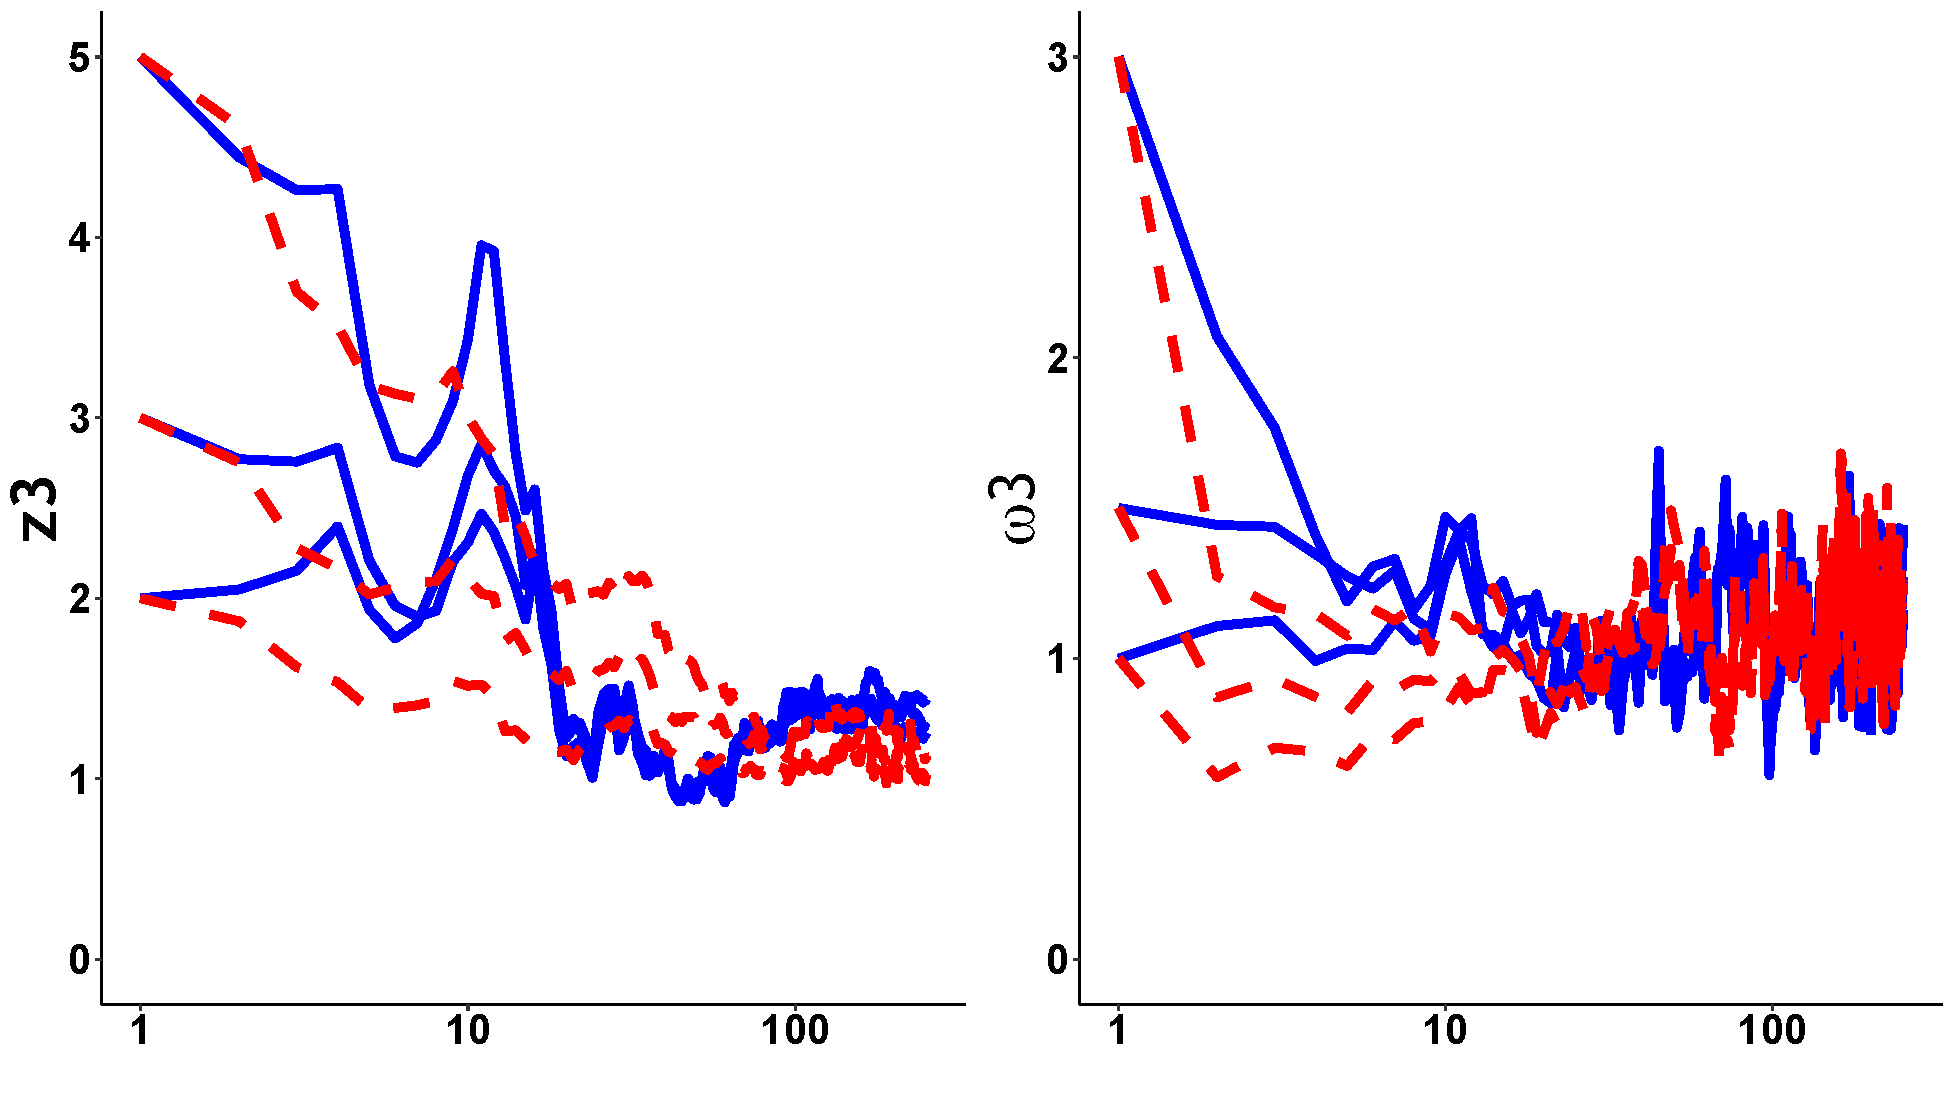
\includegraphics[scale=0.3]{pics/ordinal_imcem_final.pdf}
\caption{Convergence of the fixed parameter $z_3$ and its variance $\omega_3^2$ for the MCEM (in blue) and MBMCEM (50\%) (red)}
\label{ordinal}
\end{center}
\end{figure}

\begin{figure}[h]
\begin{center}
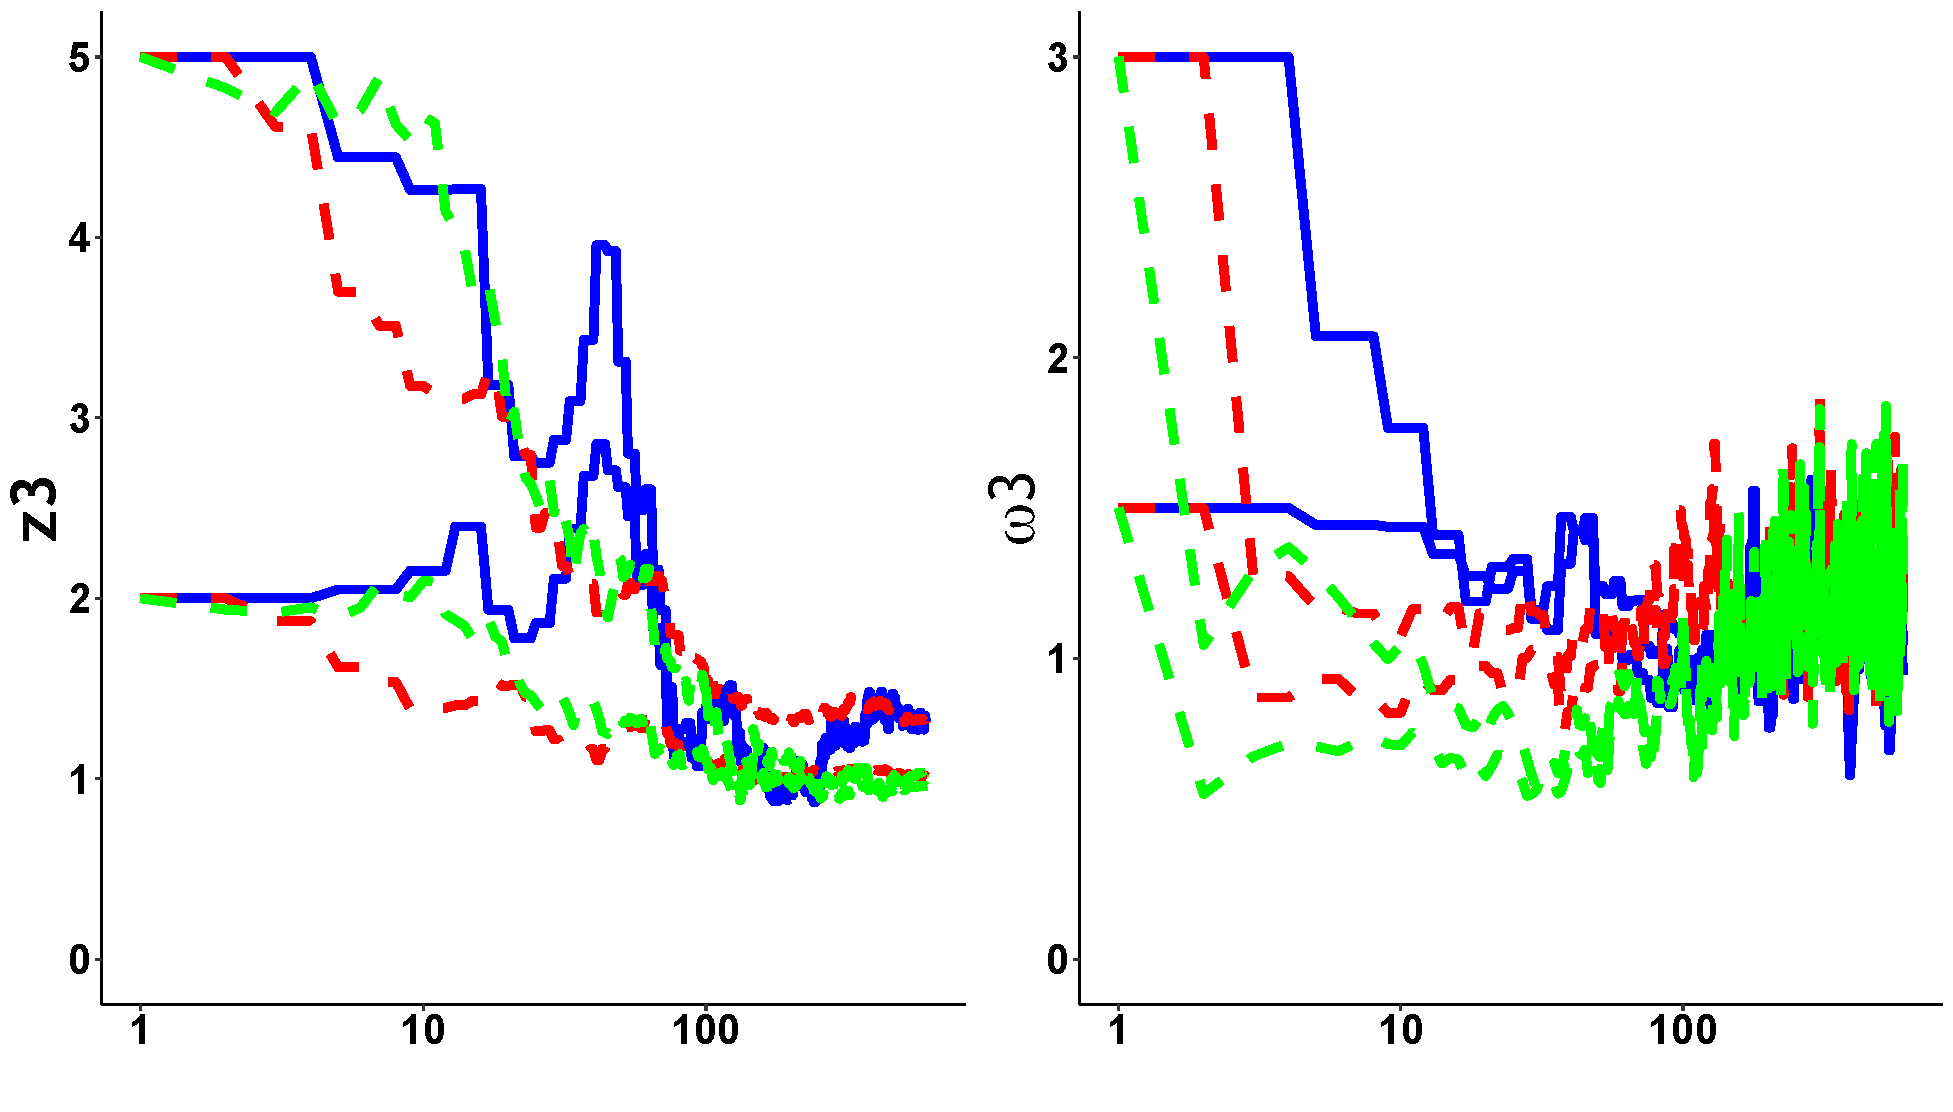
\includegraphics[scale=0.3]{pics/ordinal_severalbatch.pdf}
\caption{Convergence of the fixed parameter $z_3$ and its variance $\omega_3^2$ for the MCEM (in blue), MBMCEM (50\%) (red) and MBMCEM (25\%) (green)}
\label{ordinal}
\end{center}
\end{figure}

\clearpage
\subsubsection{A Pharmakodynamic example}

We use an example used by P. Girard and F. Mentre for the symposium dedicated to Comparison of Algorithms Using Simulated Data Sets and Blind Analysis, that took place in Lyon, France, September 2004.\\
The dataset contains 100 individuals, each receiving 3 different doses:$(0, 10, 90)$, $(5, 25, 65)$ or $(0,20, 30)$. It was assumed that doses were given in a cross-over study with sufficient wash out period to avoid carry over. Responses $y_{ij}$ were simulated with the following pharmacodynamic model:
\begin{equation}
y_{ij} = E0_i + \frac{D_{ij} Emax_i}{D_{ij} + EC50_i} +\epsilon_{ij}
\end{equation}
Where $D_{ij}$ is the dose given to individual $i$ at time $t_j$ and the individual parameters $(E0_i,Emax_i,EC50_i)$ follow log normal distribution.

\begin{figure}[h]
\begin{center}
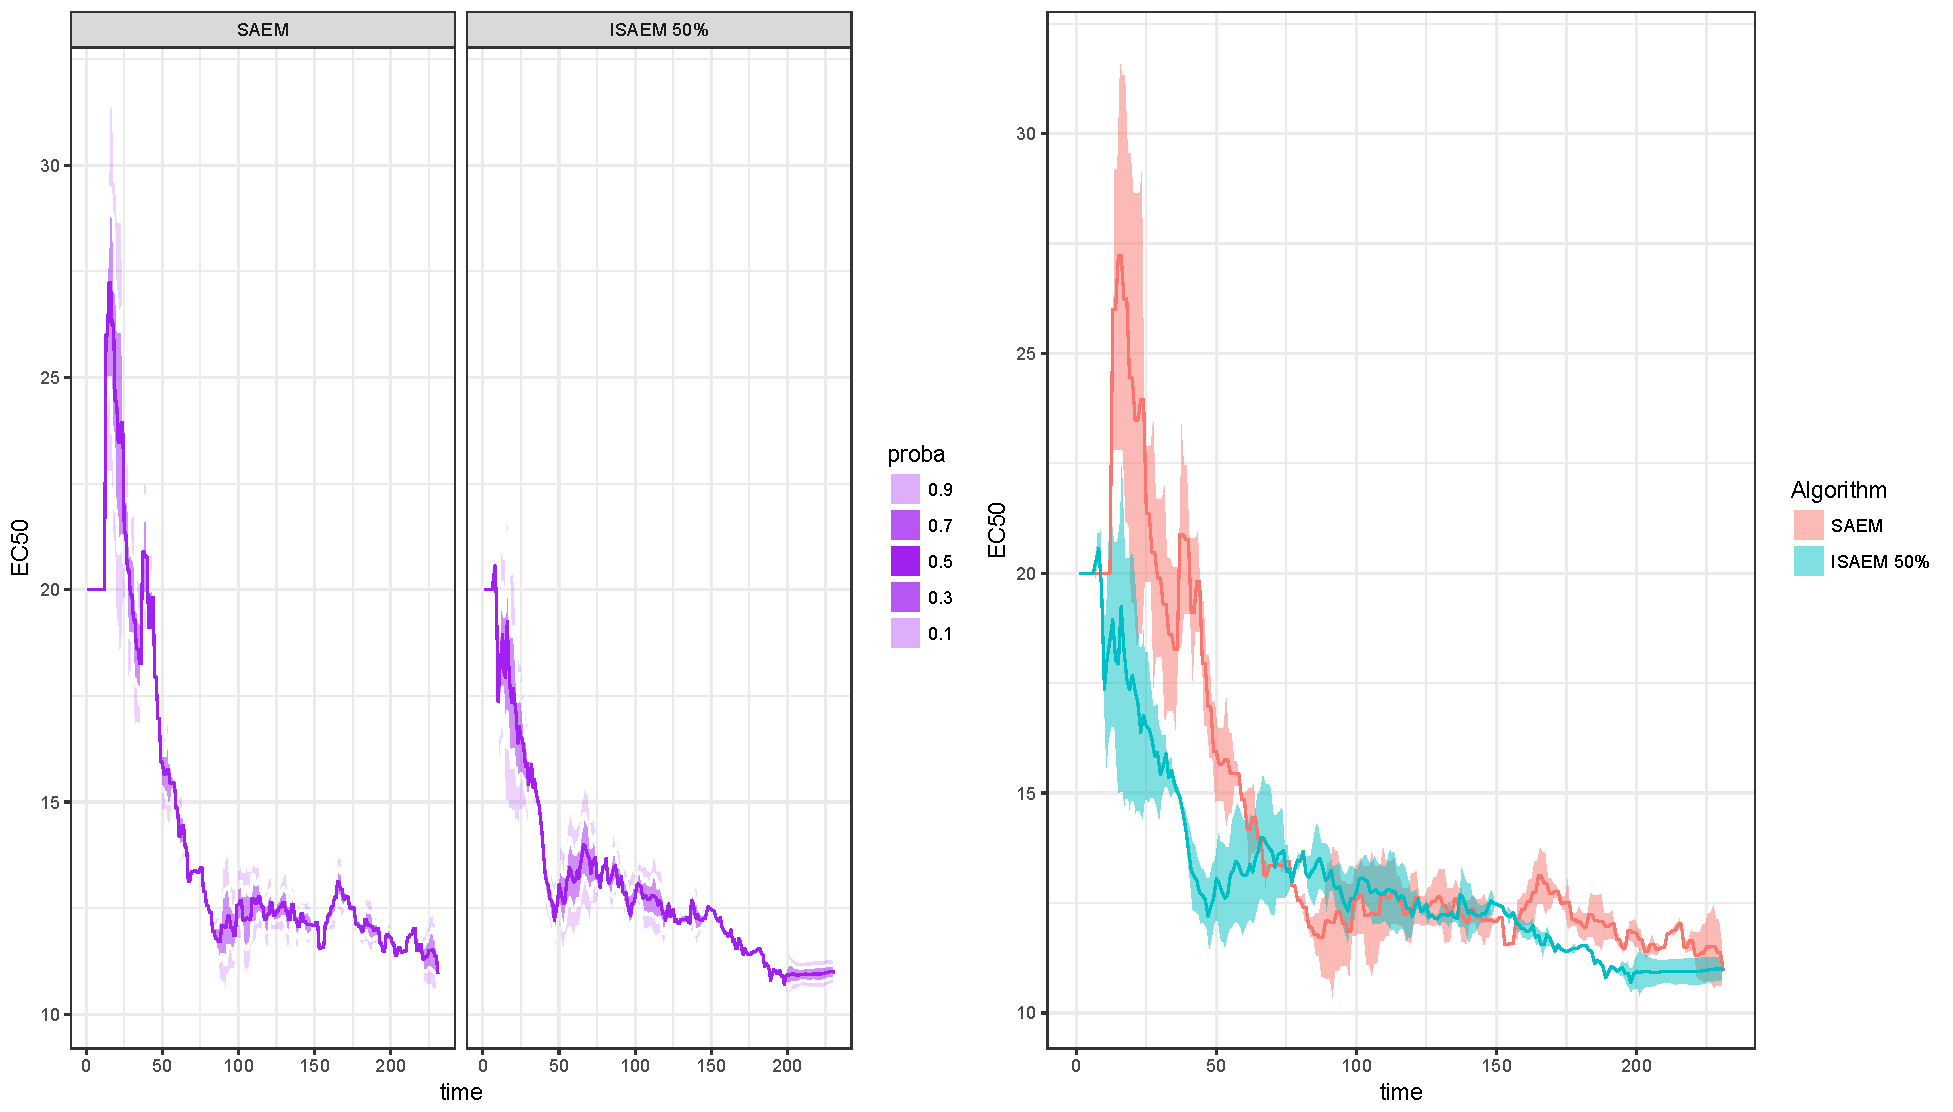
\includegraphics[scale=0.35]{isaem_pd_final.pdf}
\end{center}
\end{figure}

\section{Discussion}
\newpage
\begin{appendices}
\section{Proof of Lemma ~\ref{lemma_lypaunov}}\label{appendix:RMlemma}

Inspired by \cite{lavielle}, the whole idea behind the convergence properties relies on the expression of the mean field of the algorithm at each iteration and the proof of the existence of a Lyapunov function that satisfies SA ~\ref{assumption:lyapunov}. It is well known (see \cite{lavielle}) that the incomplete data likelihood is a Lyapunov function relative to the SAEM mapping. We'll show that this same function is a Lyapunov function relative to our new mapping.\\
Let us suppose we pick the individual $i_k$ uniformly at each iteration. Then:
\begin{equation}
\begin{split}
& i_k \sim \mathcal{U}( \inter )\\
& S_{i_k}^{k} = S_{i_k}^{k-1} + \gamma_k(\St(z_{i_k}^k)-S_{i_k}^{k-1})\\
& S_{i}^{k} = S_{i}^{k-1} \textrm{ if $i \neq i_k$}
\end{split}
\end{equation}
Which gives the $k$-th iteration of the ISAEM algorithm
\begin{equation}
S^{k} = \sum_{i=1}^{N}{S_{i}^{k} = S^{k-1} + \gamma_k(\St(z_{i_k}^k)-S_{i_k}^{k-1})
\end{equation}

Given that:
\begin{equation}
\begin{split}
& \E(\St(z_{i_k}^k)|\hat{\theta}(S^k)) = \frac{1}{N}\sum_{i=1}^{N}{\E\left(\St(z_i^k)|\hat{\theta}(S^k)\right)}\\
& \E(S_{i_k}^{k-1}|\hat{\theta}(S^k)) = \frac{1}{N}S^{k-1}
\end{split}
\end{equation}

We express the mean field of the algorithm as:
\begin{equation}
\frac{1}{N}\left(\sum_{i=1}^{N}{\E(\St(z_i^k)|\hat{\theta}(S^k))} - S^{k-1}\right)
\end{equation}


We can define the function $h$ that is the mean field of the algorithm:
\begin{equation}
h(s) = \frac{1}{N}\left(\sum_{i=1}^{N}{\E(\St(z_i)|\hat{\theta}(s))}-s \right)
\end{equation}

Let us note $l(\theta)$ and $L(s,\theta)$ the incomplete and the complete log likelihood.\\
We know that $\hat{\theta}(s)$ is a solution of the maximization of $L(s,\theta)$, so:
\begin{equation}
\begin{split}
&\partial_{\theta}L(s,\hat{\theta}(s)) = 0\\
&-\partial_{\theta}\psi(\hat{\theta}(s)) +s^t \partial_{\theta}\phi(\hat{\theta}(s)) = 0\\
\end{split}
\end{equation}
The latter expression $\partial_{\theta}L(s,\hat{\theta}(s)) = 0 $ can be differentiate with respect to the vector $s$ (under assumptions M2-M3):
\begin{equation}
\begin{split} 
& \partial^2_{\theta}L(s,\hat{\theta}(s))\partial_{s}\hat{\theta}(s) + \partial_{\theta}\phi(\hat{\theta}(s))^t = 0\\
& \partial^2_{\theta}L(s,\hat{\theta}(s))\partial_{s}\hat{\theta}(s) = -\partial_{\theta}\phi(\hat{\theta}(s))^t
\end{split}
\end{equation}

Also the Fisher identity gives:
\begin{equation}
\partial_{\theta} l(\theta) = -\int \partial_{\theta} \log p(y,z,\theta) p(z|y,\theta) \mu(\dz)
\end{equation}
written as :

\begin{equation}
\partial_{\theta} l(\theta) = \partial_{\theta}\psi(\theta) -\bar{s}^t\partial_{\theta}\phi(\theta)
\end{equation}

With the expression of the mean field of our algorithm found above, we are going to show that the scalar product of the Lyapunov function, classically considered as being the incomplete log likelihood, along the mean field is always negative or null. 
\begin{equation}
\begin{split}
& V(s) = l(\hat{\theta}(s))\\
& h(s) = \frac{1}{N}(\bar{s}(\hat{\theta}(s)) - s)
\end{split}
\end{equation}

A combination of the previous equalities gives:
\begin{equation}
\begin{split}
\frac{1}{N}\partial_{\theta} l(\hat{\theta}(s)) & = \underbrace{(\frac{1}{N}(\bar{s}-s))^t}_{h(s)}\underbrace{\partial_{\theta}\phi(\hat{\theta}(s))}_{-\partial_{s}\hat{\theta}(s)^t\partial^2_{\theta} L(s,\hat{\theta}(s))}\\
& = h(s)^t\partial_{s}\hat{\theta}(s)^t\partial^2_{\theta} L(s,\hat{\theta}(s))\\
\end{split}
\end{equation}
We can derive this expression with respect to the vector $s$. The gradient of $l(\hat{\theta}(s))$ is given by the following relation:

\begin{equation}
\begin{split}
\frac{1}{N}\partial_{s} l(\hat{\theta}(s)) & = \frac{1}{N}\partial_{\theta}l(\hat{\theta}(s))\partial_{s}\hat{\theta}(s))\\
& = h(s)^t \partial_{s}\hat{\theta}(s)^t\partial^2_{\theta} L(s,\hat{\theta}(s))\partial_{s}\hat{\theta}(s)\\
\end{split}
\end{equation}



The quantity of interest can be expressed as:

\begin{equation}
\begin{split}
F(s) = \langle \partial_{s}V(s), h(s) \rangle & = \langle \partial_{s} l(\hat{\theta}(s)), h(s) \rangle\\
& =  N h(s)^t \partial_{s}\hat{\theta}(s)^t\partial^2_{\theta} L(s,\hat{\theta}(s))\partial_{s}\hat{\theta}(s)h(s)
\end{split}
\end{equation}
As $\partial^2_{\theta} L(s,\hat{\theta}(s)) \leq 0$ we have that $\langle \partial_{s}V(s), h(s) \rangle \leq 0$ which proves the first part of ~\ref{assumption:lyapunov}.\\
Obviously, $\{s \in \mathcal{S}: \partial_{s}V(s) = 0\} \subset \{s \in \mathcal{S}: F(s) = 0\}$.\\ If $s^* \in \{s \in \mathcal{S}: F(s) = 0\}$ then:
\begin{equation}
\begin{split}
F(s^*) & = N h(s)^t \partial_{s}\hat{\theta}(s^*)^t\partial^2_{\theta} L(s^*,\hat{\theta}(s^*))\partial_{s^*}\hat{\theta}(s^*)h(s^*)\\
& = \langle \partial_{s} l(\hat{\theta}(s)), h(s) \rangle = 0
\end{split}
\end{equation}
Since $\partial^2_{\theta} L(s^*,\hat{\theta}(s^*))$ is non positive then $\partial_{s} l(\hat{\theta}(s^*)) = 0$ which proves $\partial_{s}V(s^*) = 0$ and the reverse inclusion.\\
Using Sard's theorem, in \cite{brocker}, we have that $V(\{s \in \mathcal{S}, \partial_s V(s) = 0 \})$ has zero Lebesgue measure which proves the second part of ~\ref{lemma_lypaunov}.

\clearpage
\section{Proof of Theorem ~\ref{rmtheo}}\label{appendix:rmtheo}
We prove the results on a sample path by sample path basis. In all the statements below, the qualifier ``w.p.1'' is implicit. The function F is upper semicontinuous and nonpositive, the set $\mathcal{L} \triangleq \{s \in \mathcal{S}: F(s)=0 \}$. Define:

\begin{equation}
s'_n = s_n + \sum_{i=n+1}^{\infty}{\gamma_i e_i}
\end{equation}

Which gives the following RM update:

\begin{equation}
s'_n = s'_{n-1} + \gamma_n h(\s_{n-1}) + \gamma_n r_n
\end{equation}

Condition (SA3) implies that there exists a compact set $\mathcal{K} \subset \mathcal{H}$ such that $s_n \in \mathcal{K}$, for all $n \geq 0$ (note that this compact set depends upon the trajectory). For $\alpha > 0$, define $\mathcal{K}_{\alpha} = \{s \in \mathbb{R}^m: d(s,\mathcal{K}) \leq \alpha\}$, where $d(s,\mathcal{K})$ is the distance from $s$ to $\mathcal{K}$.\\
Since $\mathcal{H}$ is an open subset, there exists $\rho > 0$ such that $\mathcal{K}_{\rho} \subset \mathcal{H}$. Also $\sum_{i=n+1}^{\infty}{\gamma_i e_i} \to 0$ and $r_n \to 0$ and the mean field being bounded by assumption we have:

\begin{equation}
||s'_n - s'_{n-1}|| = \mathcal{O}(\gamma_n )
\end{equation}

and the segment $\[s'_n,s'_{n-1}\] \subset \mathcal{K}_{\rho}$ for $n$ large enough.
The Lyapunov function V is continuously differentiable on $ \mathcal{H$ . For $n$ sufficiently large, there exists $s''_{n-1} \in \[s'_n,s'_{n-1}\] $ such that:

\begin{equation}
\begin{split}
V(s'_n) & = V(s'_{n-1}) +  \langle \partial_sV(s'_{n-1}),(s'_n-s'_{n-1}) \rangle\\
& = V(s'_{n-1}) + \gamma_n F(s'_{n-1}) + \gamma_n r'_n
\end{split}
\end{equation}
With $r'_n= \langle \partial_sV(s'_{n-1}),h(s_{n-1})-h(s'_{n-1}) \rangle + \langle \partial_sV(s''_{n-1})-\partial_sV(s'_{n-1}),h(s_{n-1}) \rangle + \langle \partial_sV(s''_{n-1}),r_n \rangle$

Since $h$ and $\partial_s V(s)$ are continuous on $\mathcal{K}_{\rho}$ and $\mathcal{K}_{\rho}$ is compact then $h$ and $\partial_s V(s)$ are uniformly continuous on $\mathcal{K}_{\rho}$, thus $r'_n = o(1)$ and 
\begin{equation}
V(s'_n) = V(s'_{n-1}) + \gamma_n F(s'_{n-1}) + o(\gamma_n)
\end{equation}

The following proof proceed in two steps. First proving the convergence of $\{V(s'_n)\}_{n \geq 0}$ to some point $V^*$. The second step consists in proving the convergence of the sequence $\{s'_n\}_{n \geq 0}$ to a connected component of $\mathcal{L}$.\\

\noindent \texttt{STEP 1.} For $\alpha > 0$, define $\mathcal{A}_{\alpha} = \{x \in \mathbb{R}^m: d(x,V(\mathcal{L} \cap \mathcal{K}_{\rho})) \leq \alpha\}$. Here $V(\mathcal{L} \cap \mathcal{K}_{\rho})$ is a compact subset of $\mathbb{R}$ and $\mathcal{A}_{\alpha}$ is compact; $\mathcal{A}_{\alpha}$ is a finite union of disjoint closed intervals.

\begin{equation}
\mathcal{A}_{\alpha} = \cup_{i=1}^{N_{\alpha}}[a_{\alpha}^{(i)}, b_{\alpha}^{(i)}]
\end{equation}
With $a_{\alpha}^{(1)} < b_{\alpha}^{(1)} < a_{\alpha}^{(2)} < \dots < b_{\alpha}^{(N_{\alpha})}$. Let us define $\mathcal{N}_{\alpha} = V^{-1}[\mathcal{A}_{\alpha}]$ that is an open neighborhood of the set $\mathcal{L} \cap \mathcal{K}_{\rho}$ since $V$ is continuous. Since F is upper semicontinuous (any upper semicontinuous function reaches its maximum on any compact set), there exists $\epsilon_{\alpha} > 0$ such that for n sufficiently large:

\begin{equation}
s'_n \in \mathcal{K}_{\alpha} \backslash \mathcal{N}_{\alpha} \Rightarrow F(s'_{n-1}) \leq -2 \epsilon_{\alpha}
\end{equation}
Which implies:

\begin{equation}\label{lyap_io}
V(s'_n) \leq V(s'_{n-1}) - \gamma_n \epsilon_{\alpha} + \gamma_n (C_V +\epsilon_{\alpha})(V(s'_{n-1}) \in int(\mathcal{A}_{\alpha}))
\end{equation}
Since $\sum{\gamma_n} = \infty$, this last equation implies that  $\{V(s'_n)\}_{n \geq 0}$ is infinitely often in $\mathcal{A}_{\alpha}$. Here $\mathcal{A}_{\alpha}$ is a finite union of disjoint intervals, thus $\{V(s'_n)\}_{n \geq 0}$ is infinitely often in a given interval that compose the set $\mathcal{A}_{\alpha}$. Let us call this interval $[a_{\alpha}, b_{\alpha}]$.\\
Let $\delta > 0$ be such that  $[a_{\alpha} - 2\delta , b_{\alpha} +2\delta] \cap \mathcal{A}_{\alpha} =  [a_{\alpha} b_{\alpha}]$  (such $\delta$ exists because $\mathcal{A}_{\alpha}$ is a finite union of closed disjoints intervals), and let $N_V$ be such that, for all $n \geq N_V$, $\gamma_n \leq \delta/C_V$.\\
Finally, let $N$ be the first index greater than $N_V$ such that $V(s′_N) \in  [a_{\alpha}, b_{\alpha}]$  (such index exists because $V(s′_N)$  is i.o. in $[a_{\alpha}, b_{\alpha}]$).
The equation ~\ref{lyap_io} implies that, for all $n \geq N$, $V(s'_n) \in [a_{\alpha} - \delta, b_{\alpha} + \delta]$.\\
Hence, $\delta$ being arbitrary, the set of limit points $\mathcal{V}$ of the sequence $\{V(s'_n)\}_{n \geq 0}$ is included in the interval $[a_{\alpha}, b_{\alpha}]$.\\
If we now take $\alpha' < \alpha$, we can proceed as above and show that  $\mathcal{V} \subset [a_{\alpha'}, b_{\alpha'}]$ with $[a_{\alpha'}, b_{\alpha'}]$ interval element of the union of disjoint intervals of $\mathcal{A}_{\alpha'}$.\\
We apply the above result with a non increasing sequence $\alpha_n$ that tends to zero and with of course $[a_{\alpha_{n}}, b_{\alpha_{n}}] \subset [a_{\alpha_{n-1}, b_{\alpha_{n-1}}]$.
We can thus show that $\mathcal{V}$ is included in the intersection of a decreasing sequence of closed intervals $[a_{\alpha_{n}, b_{\alpha_{n}}]$, and thus $\mathcal{V}$ is itself a closed interval.
Since all the intervals $[a_{\alpha_{n}, b_{\alpha_{n}}]$ are included in $\mathcal{A}_{\alpha_{n}}$ and $\cap_{n} \mathcal{A}_{\alpha}= V(\mathcal{L}\cap \mathcal{K}_{\rho})$ then $\mathcal{V}$ is also a subset of $V(\mathcal{L}\cap \mathcal{K}_{\rho})$.
The set $V(\mathcal{L}\cap \mathcal{K}_{\rho})$ has an empty interior and the connected components of $V(\mathcal{L}\cap \mathcal{K}_{\rho})$ are reduced to points.\\
Since $\mathcal{V}$ is connected, it must be reduced to a point which implies that $\lim \limits_{n \to \infty} V(s'_n)$ exists. 
Finally, since $\lim \limits_{n \to \infty} V(s_n) = \lim \limits_{n \to \infty} V(s'_n)$ we prove the convergence of $\{V(s_n)\}_{n \geq 0}$.\\

\noindent \texttt{STEP 2.} Let $\mathcal{N}$ be an arbitrary open neighborhood of $\mathcal{L}$. There exists $\epsilon_{\mathcal{N}} > 0$ such that for $n$ sufficiently large:

\begin{equation}\label{lyap_io}
V(s'_n) \leq V(s'_{n-1}) - \gamma_n \epsilon_{\mathcal{N}} + \gamma_{\mathcal{N}} (C_V +\epsilon_{\mathcal{N}})\indic(s'_{n-1} \in\mathcal{N})
\end{equation}

Since $\{V(s'_n)\}_{n \geq 0}$ converges and $\gamma_n = o(1)$
, for any $\tau > 0$, there exists $N_{\tau} < \infty$ such that:
\begin{equation}
\begin{split}
& |V(s'_n) -V(s'_p)| \leq \tau \\
& N_{\tau} \leq n \leq p \\
& \gamma_k < \frac{\tau}{\epsilon_{\mathcal{N}}}\\
& N_{\tau} \leq k
\end{split}
\end{equation}

We obtain that:
\begin{equation}
\epsilon_{\mathcal{N}} \sum_{k=n+1}^{p}{\gamma_k - (C_V +\epsilon_{\mathcal{N}})}\sum_{k=n+1}^{p}{\gamma_k \indic(s'_{k-1} \in\mathcal{N})} \leq \tau
\end{equation}

Choose $n \geq N_{\tau}$ and let $p(n)$ be the first integer larger than $n$ such that:

\begin{equation}
\frac{\tau}{\epsilon_{\mathcal{N}}} <  \sum_{k=n+1}^{p(n)}{\gamma_k}< 2\frac{\tau}{\epsilon_{\mathcal{N}}}
\end{equation}

Thus, there exists $k(n) \in [n, p(n)]$ such that $s'_{k(n)} \in \mathcal{N}$.
Since $||s'_n - s'_{n-1}|| = \mathcal{O}(\gamma_n )$ then there exists a finite constant $K$ such that, for all $n \geq 1$, $||s'_n - s'_{n-1}|| \leq K \gamma_n$ which yields to:

\begin{equation}
||s'_{k(n)} - s'_{n-1}|| \leq K \sum_{l=n+1}^{k(n)}{\gamma_l}\leq K \sum_{l=n+1}^{p(n)}{\gamma_l} \leq 2K \frac{\tau}{\epsilon_{\mathcal{N}}}
\end{equation}

By construction, $s'_{k(n)} \in \mathcal{N}$ and the last relation implies that $d(s'_n, clos(\mathcal{N})) \leq 2K \frac{\tau}{\epsilon_{\mathcal{N}}}$. Since $\tau$ is chosen arbitrarily we have that:
\begin{equation}
\lim \limits_{n \to \infty} d(s'_n, \mathcal{N}) = 0
\end{equation}

$\mathcal{N}$ being arbitrary, we have that $\{s'_n\}_{n \geq 0}$ tends to $\mathcal{L}$ and so does $\{s_n\}_{n \geq 0}$.\\
The set of limit points of $\{s_n\}_{n \geq 0}$ is compact because it is bounded and closed and since $||s'_n - s'_{n-1}|| = \mathcal{O}(\gamma_n )$, it is connected and $||s'_n - s'_{n-1}|| \to 0$. Which proves the convergence of the sequence $\{s_n\}_{n \geq 0}$.

\clearpage

\section{Proof of Theorem ~\ref{theorem_isaem}}\label{appendix:ISAEM}
First of all, we verify assumptions of Theorem 2. (SA1) is verified under (IEXPO 1) and (ISAEM1) because the stepsize $\gamma_k$ is strictly inferiror to 1 and the convex hull of $\St(\mathbb{R}^p)$ is in $\mathcal{S}$. (SA4) is implied by (ISAEM1) and (SA5) by (ISAEM4). Note that under (A), there exists w.p.1 a compact set $\mathcal{K}$  , such that $s_k \in \mathcal{K}$ for all $k \geq 0$. Denote $M_n =  \sum_{k=1}^{n}{\gamma_kE_k}$. Then  $\{M_n\}_{n \geq 1}$ is a  martingale which satisfies, under (ISAEM1)–(ISAEM3):

\begin{equation}
\begin{split}
\sum_{n=1}^{\infty}{\E{\left[||   M_{n+1}-M_n||^2 | \mathcal{F}_n\right]}} & = \sum_{n=1}^{\infty}{\E{\left[||\gamma_{n+1}E_{n+1} ||^2| \mathcal{F}_n \right]}}\\
& \leq \sum_{n=1}^{\infty}{\gamma_{n+1}^2 \int{||\St(y_{i_k},z_{i_k}^k)||^2 p(z_{i_k}|y_{i_k},\hat{\theta}(s_k))}} \\
& - \sum_{n=1}^{\infty}{\gamma_{n+1}^2 \int{||\St(y_{i_k},z_{i_k}^{k-1})||^2 p(z_{i_k}|y_{i_k},\hat{\theta}(s_k))}} < \infty
\end{split}
\end{equation}

This proves the existence of $\lim \limits_{n \to \infty} M_n$ (see Hall and Heyde (1980) Theorem 2.15 p.33).\\
We can apply Lemma ~\ref{lemma_lypaunov} which proves (SA3) and finally Theorem ~\ref{rmtheo} can be applied which results in, w.p.1:
\begin{equation}
d(\theta^k, \mathcal{L}) \to 0
\end{equation}

The second part of the Theorem is proved by applying Lemma ~\ref{lemma_lypaunov}.

\end{appendices}
\newpage

\printbibliography 
\end{document}